\documentclass[journal=jcisd8,manuscript=article]{achemso}

\usepackage{amsmath,amssymb,amsfonts}
\usepackage{graphicx}
\graphicspath{{figures/}{./}}
\usepackage{booktabs}
\usepackage{tabularx}
\usepackage{multirow}
\usepackage{xcolor}
\usepackage{hyperref}

\hypersetup{
    colorlinks=true,
    linkcolor=blue,
    citecolor=blue,
    urlcolor=blue
}

\title{Predicting Iron--Sulfur Protein Reduction Potentials Using a pH-Conditioned Multi-Relational Residue Graph Neural Network}

\author{[AUTHOR LIST ANONYMIZED FOR PEER REVIEW]}
\affiliation{[INSTITUTION ANONYMIZED FOR PEER REVIEW]}
\email{[CORRESPONDING AUTHOR EMAIL]}

\begin{document}

\begin{abstract}
The midpoint reduction potentials ($E_m$) of iron--sulfur (Fe--S) proteins span an extraordinary $\sim 1000\text{ mV}$ physiological range governed by secondary-sphere electrostatics, hydrogen-bonding networks, and solvent pH. Here, we present FiLM-RGCN, a pH-conditioned multi-relational residue graph neural network that represents protein structures using five biophysical contact types and modulates intermediate convolutional representations by experimental solvent pH via Feature-wise Linear Modulation. Evaluated on a curated benchmark of 364 experimentally characterized Fe--S proteins across 76 crystal scaffolds, the relative performance of graph and tabular models depends strongly on the validation regime. Under standardized random 5-fold cross-validation, a curated 96-descriptor XGBoost baseline outperforms FiLM-RGCN ($48.39 \pm 3.98\text{ mV}$ versus $57.83 \pm 6.46\text{ mV}$ MAE). However, when evaluated under PDB-grouped cross-validation (preventing base-scaffold co-occurrence), FiLM-RGCN achieves a lower error ($83.82 \pm 16.38\text{ mV}$ versus $96.20 \pm 27.29\text{ mV}$). Under sequence-homology-held-out cross-validation ($<30\%$ pairwise sequence identity), FiLM-RGCN reports an MAE of $109.18 \pm 43.82\text{ mV}$ ($R^2 = 0.654$, $r = 0.820$), compared to $151.59 \pm 25.53\text{ mV}$ ($R^2 = 0.474$, $r = 0.717$) for XGBoost. Conversely, out-of-fold prediction of 233 point-mutation shifts ($\Delta E_m$) exhibits poor directional sign accuracy ($42.5\%$) and a scaffold-bootstrap 95\% confidence interval for correlation spanning zero ([$ -0.198, 0.683$]), identifying mutational polarity as a key operational boundary.
\end{abstract}

\section{Introduction}

Iron--sulfur (Fe--S) metalloproteins are essential electron-transfer catalysts in biological respiration, photosynthesis, nitrogen fixation, and genome maintenance.\cite{beinert1997iron,holm1996structural,cammack1992iron,johnson1998iron,lill2006iron} Despite sharing common inorganic cores---predominantly $[2\text{Fe}--2\text{S}]$, $[4\text{Fe}--4\text{S}]$, $[3\text{Fe}--4\text{S}]$, and mononuclear rubredoxin $[1\text{Fe}]$ centers---their experimental midpoint reduction potentials ($E_m$) span an extraordinary physiological continuum from below $-700\text{ mV}$ in low-potential bacterial ferredoxins to above $+350\text{ mV}$ in high-potential iron proteins (HiPIPs) and Rieske-type centers.\cite{beinert1997iron,stephens1996protein,cowan1993metalloprotein} Modulating these potentials directly alters electron-transfer thermodynamics and metabolic pathways,\cite{marcus1993electron,moser1992nature,marshall2009rationally} making the computational prediction of Fe--S reduction potentials from structural data an important goal in computational bioinorganic chemistry.

Predicting $E_m$ directly from coordinate data is challenging because the macroscopic potential is not determined solely by the immediate primary coordination sphere.\cite{stephens1996protein,niu1999theoretical} Instead, $E_m$ is tuned by subtle, cooperative interactions throughout the surrounding protein microenvironment. Key contributing factors include the spatial arrangement of coordinating ligands, backbone and side-chain $\text{N}--\text{H}\cdots\text{S}$ hydrogen-bonding interactions that stabilize accumulated negative charge upon reduction,\cite{adman1975hydrogen,carter1977iron,swartz1996structural} local dielectric screening and solvent accessibility,\cite{kassner1972effects,churg1986dielectric,honig1995classical} and through-space electrostatic interactions with polar or charged residues.\cite{rees1980experimental} Furthermore, experimental redox measurements are coupled to environmental solvent pH via proton-coupled electron transfer (PCET) or the titration of nearby ionizable residues.\cite{huynh2007proton,zu2001complete,zu2003reduction}

Quantum-chemical cluster calculations,\cite{mouesca1994density,noodleman2004quantum} continuum Poisson--Boltzmann models,\cite{ullmann2002density,torres2003density} and hybrid QM/MM simulations\cite{niu1999theoretical,mancuso2018minimal} have provided valuable physical insights into Fe--S redox chemistry. However, these methods remain computationally expensive and sensitive to setup parameters, limiting their throughput for large-scale structural screening. Recently, machine learning approaches have been explored. Persico et al.\ developed FeS-RedPred,\cite{persico2025predicting} combining engineered biophysical descriptors with Extreme Gradient Boosting (XGBoost)\cite{chen2016xgboost} to predict Fe--S redox potentials across a unified structural collection. While tabular models based on aggregated scalar features can achieve low errors when test examples closely resemble training examples, fixed spatial aggregation compresses directional geometry into static summaries and can degrade when applied to unfamiliar protein folds where spatial arrangements diverge from the training distribution.

Graph neural networks (GNNs) provide an alternative framework by representing macromolecular structures as graphs with residues as nodes and biophysical interactions as edges.\cite{scarselli2008graph,kipf2017semi,gilmer2017neural,dauparas2022robust,jing2021learning,jumper2021highly} However, standard isotropic GNNs treat all spatial proximities uniformly, risking the dilution of distinct biochemical signals. A multi-relational graph convolutional network (RGCN)\cite{schlichtkrull2018modeling} addresses this by assigning relation-specific transformation parameters to different interaction types. Furthermore, because environmental pH modulates reduction potentials, intermediate neural representations can be conditioned on solvent pH using Feature-wise Linear Modulation (FiLM).\cite{perez2018film}

In this work, we present FiLM-RGCN, a pH-conditioned multi-relational residue graph neural network for Fe--S protein reduction potential prediction. We evaluate the model against a curated tabular XGBoost baseline across three validation regimes: random cross-validation, scaffold-held-out cross-validation, and sequence-homology-held-out cross-validation ($<30\%$ pairwise sequence identity). Our central finding is that while XGBoost performs better under random-split interpolation, FiLM-RGCN demonstrates superior generalization when base-scaffold and sequence-homology leakage are eliminated. We also evaluate the model's sensitivity to structural edge perturbations and out-of-fold point-mutation shifts, establishing both the predictive capabilities and the clear operational limits of the current architecture.

\section{Methods}

\subsection{Dataset Curation and Nuclearity Breakdown}
The experimental dataset analyzed in this study is based on the Fe--S redox potential collection compiled by Persico et al.,\cite{persico2025predicting} derived from structures deposited in the Protein Data Bank (PDB)\cite{berman2000protein} and documented experimental potentials ($E_m$ in mV versus SHE). In accordance with reporting guidelines for machine learning in structural biology (DOME),\cite{walsh2021dome} the dataset was audited for completeness. 

The curated benchmark comprises exactly $N = 364$ complete observations across 76 unique base crystal scaffolds, with zero missing values across all descriptor columns and target variables. The dataset contains 131 wild-type (WT) proteins ($36.0\%$) and 233 site-directed mutational variants ($64.0\%$). Experimental potentials span an $890\text{ mV}$ range ($-500.0\text{ mV}$ to $+390.0\text{ mV}$, mean $\pm$ standard deviation: $-103.7 \pm 245.9\text{ mV}$), with solvent pH values ranging from 3.00 to 14.00 ($7.15 \pm 1.79$). 

Structural inspection revealed four cluster nuclearity classes:
\begin{itemize}
    \item $[2\text{Fe}--2\text{S}]$ ferredoxins: 293 observations ($80.5\%$) across 61 base scaffolds;
    \item Rubredoxin $[1\text{Fe}]$ centers: 52 observations ($14.3\%$) across 7 base scaffolds;
    \item $[4\text{Fe}--4\text{S}]$ clusters: 11 observations ($3.0\%$) across 5 base scaffolds;
    \item $[3\text{Fe}--4\text{S}]$ clusters: 8 observations ($2.2\%$) across 3 base scaffolds.
\end{itemize}
The distribution is heavily dominated by $[2\text{Fe}--2\text{S}]$ proteins. All entries were retained, and performance was evaluated across stratified subgroups.

\subsection{Multi-Relational Residue Graph Representation}
Each protein structure is represented as a molecular graph $\mathcal{G} = (\mathcal{V}, \mathcal{E}, \mathcal{R})$ constructed from atomic coordinates. Nodes $i \in \mathcal{V}$ represent standard amino acid residues positioned at their $\text{C}_\alpha$ coordinates. The active Fe--S center centroid $\mathbf{c}_{\text{FeS}} \in \mathbb{R}^3$ was calculated as the arithmetic mean of all resolved inorganic iron and sulfur atoms (or cysteine-coordinated iron atoms for rubredoxins):
\begin{equation}
\mathbf{c}_{\text{FeS}} = \frac{1}{M} \sum_{m=1}^M \mathbf{r}_m
\end{equation}
For each residue $i$, the Euclidean distance to the cofactor centroid is $d_i = \|\mathbf{r}_{i,\text{C}\alpha} - \mathbf{c}_{\text{FeS}}\|_2$. The Fe--S cluster itself is not represented as an explicit graph node.

\subsubsection{Node Features}
Each residue node $i$ is assigned a 49-dimensional feature vector $\mathbf{x}_i \in \mathbb{R}^{49}$:
\begin{enumerate}
    \item A 20-dimensional one-hot indicator of standard amino acid identity;
    \item A 28-dimensional vector of normalized physicochemical descriptors (including molecular weight, van der Waals volume, hydrophobicity scales, isoelectric point, and side-chain charge; details in Supporting Information);
    \item A 1-dimensional near-cofactor cysteine indicator set to $1.0$ if the residue is Cys with $d_i < 6.5\text{ \AA}$, and $0.0$ otherwise. This is an approximate spatial heuristic and does not explicitly identify non-cysteine coordinating ligands (e.g., histidines in Rieske centers).
\end{enumerate}

\subsubsection{Relational Edge Construction}
Edges are categorized into five distinct interaction types ($\mathcal{R} = \{0, 1, 2, 3, 4\}$):
\begin{itemize}
    \item \textbf{Type 0 (Sequential Backbone):} Directed bonds between adjacent residues along the polypeptide chain with $\|\mathbf{r}_{i+1,\text{C}\alpha} - \mathbf{r}_{i,\text{C}\alpha}\|_2 \le 4.2\text{ \AA}$;
    \item \textbf{Type 1 (Spatial Contacts):} Distance-defined non-bonded proximities between non-adjacent residues with $0.1\text{ \AA} < \|\mathbf{r}_{i,\text{C}\alpha} - \mathbf{r}_{j,\text{C}\alpha}\|_2 \le 8.0\text{ \AA}$;
    \item \textbf{Type 2 (Putative Polar Contacts):} Putative hydrogen-bond candidates defined by interatomic distance $\|\mathbf{r}_{i,\text{N}} - \mathbf{r}_{j,\text{O}}\|_2 \le 3.5\text{ \AA}$ ($i \neq j$) without explicit donor--hydrogen--acceptor angular geometry [VERIFY GRAPH EDGE IMPLEMENTATION];
    \item \textbf{Type 3 (Cysteine Proximity Contacts):} Close contacts between cysteine side-chain sulfur atoms with $\|\mathbf{r}_{i,\text{S}\gamma} - \mathbf{r}_{j,\text{S}\gamma}\|_2 \le 2.5\text{ \AA}$ (these represent proximate sulfur atoms and do not explicitly encode metal--sulfur coordinate bonds);
    \item \textbf{Type 4 (Salt Bridges):} Electrostatic contacts between basic residues (Arg, Lys, His) and acidic residues (Asp, Glu) with $\|\mathbf{r}_{i,\text{C}\alpha} - \mathbf{r}_{j,\text{C}\alpha}\|_2 \le 6.0\text{ \AA}$.
\end{itemize}

\begin{figure}[htbp]
\centering
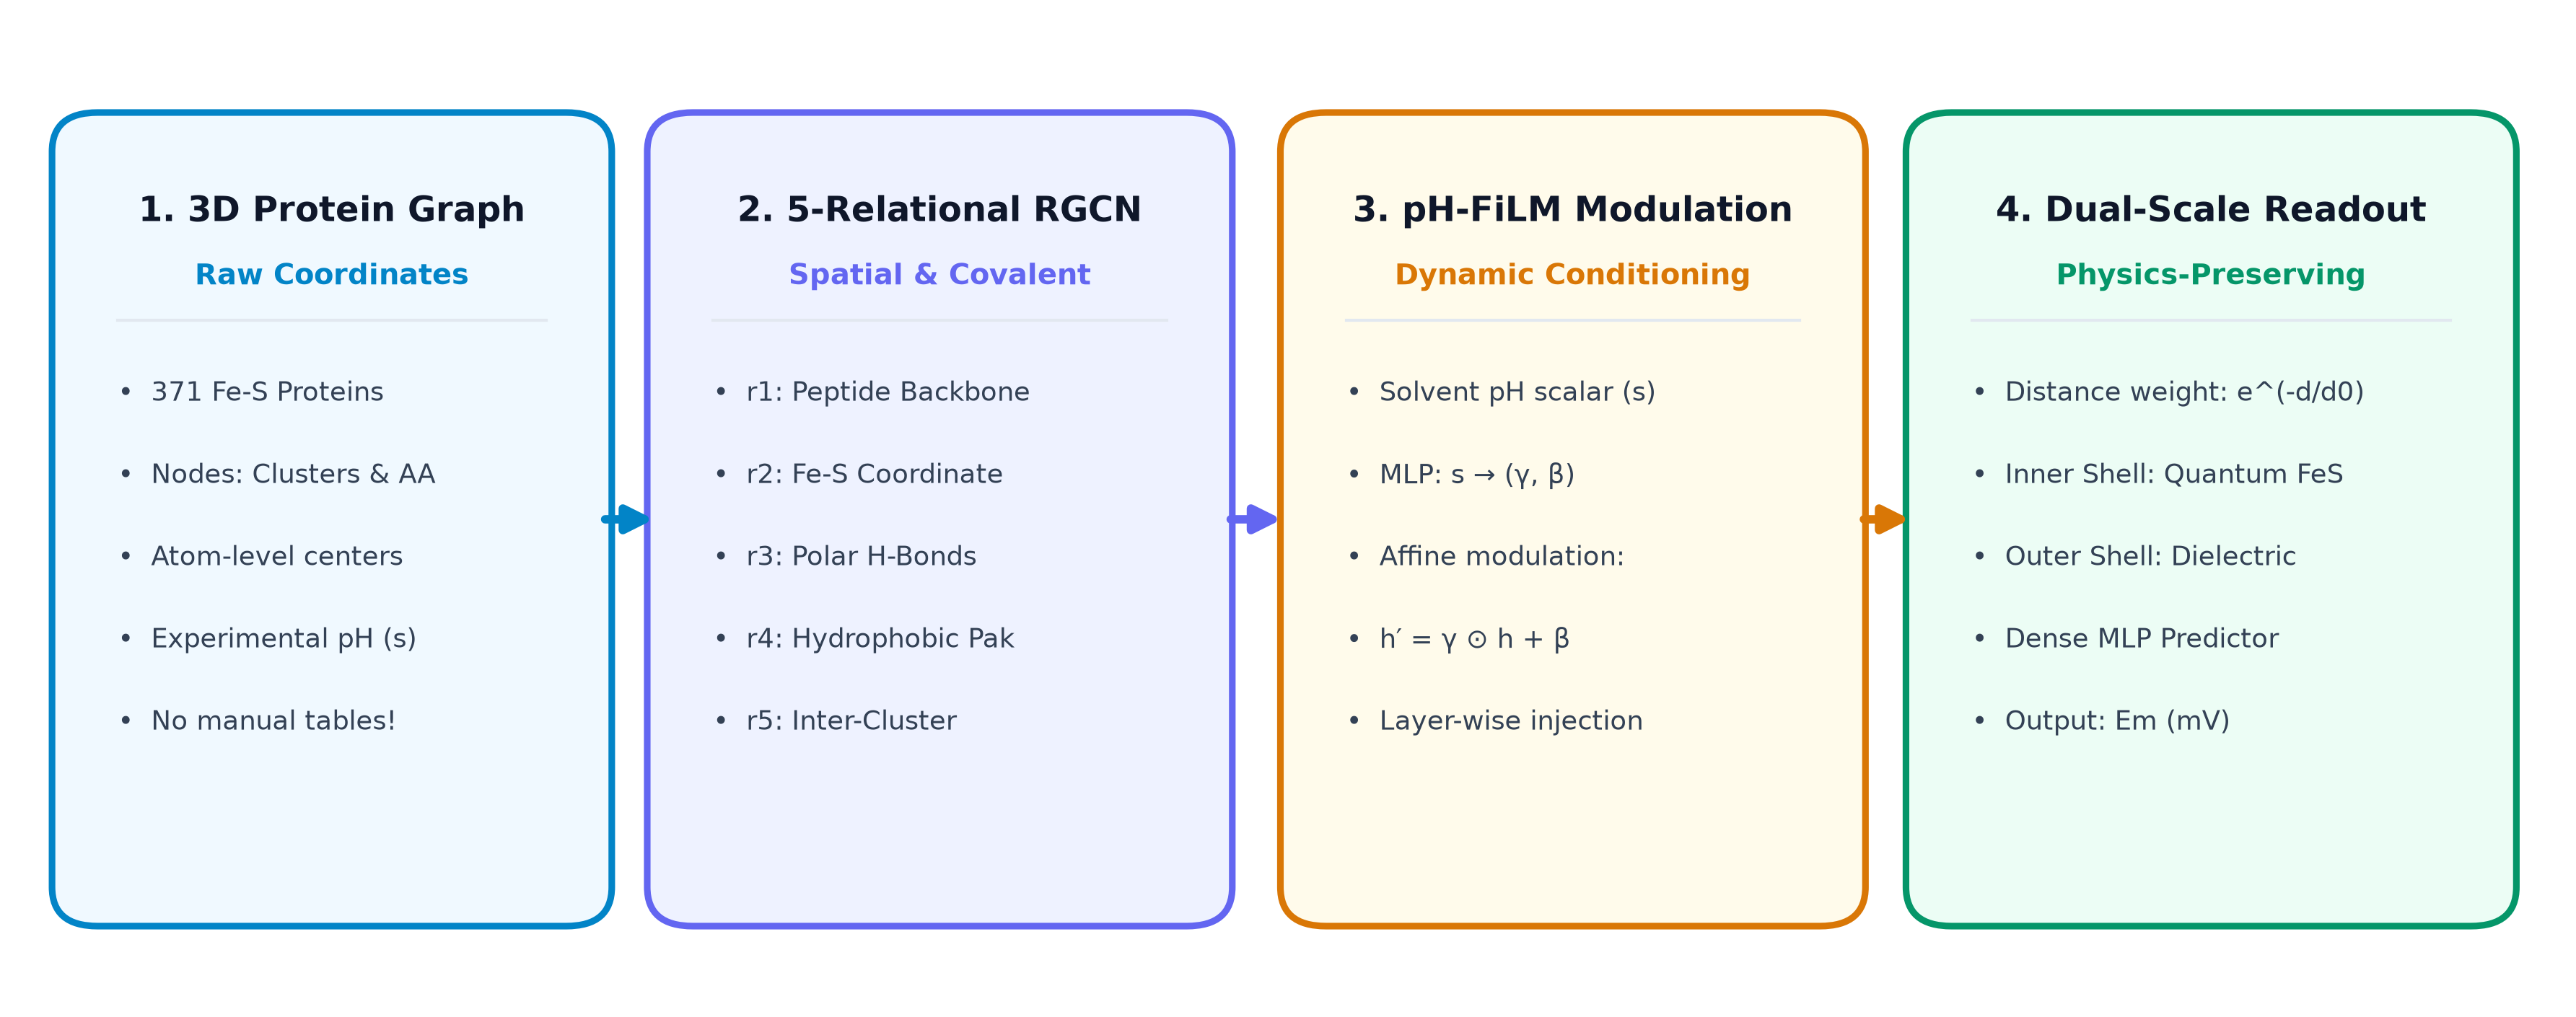
\includegraphics[width=\textwidth]{fig1_workflow_architecture.png}
\caption{Overview of the FiLM-RGCN residue-level architecture. (A) Structural coordinates and calculation of the Fe--S cofactor spatial centroid. (B) Construction of multi-relational residue graphs across five structural contact types. (C) Layer-wise Feature-wise Linear Modulation (FiLM) conditioned on normalized solvent pH. (D) Dual-scale Fe--S-centered radial distance readout predicting midpoint reduction potential $E_m$.}
\label{fig:workflow}
\end{figure}

\subsection{FiLM-RGCN Architecture and pH Conditioning}
The model consists of an input linear projection, $L=2$ relational graph convolutional layers with layer-wise FiLM modulation, and a dual-scale radial readout head (Figure~\ref{fig:workflow}).

Initial features $\mathbf{x}_i \in \mathbb{R}^{49}$ are projected into hidden dimension $h=7$:
\begin{equation}
\mathbf{h}_i^{(0)} = \text{LeakyReLU}\left(\mathbf{W}_{\text{in}} \mathbf{x}_i + \mathbf{b}_{\text{in}}\right)
\end{equation}

\subsubsection{Relational Message Passing}
At each layer $l \in \{0, 1\}$, message passing across the five relation types is governed by Relational Graph Convolution:\cite{schlichtkrull2018modeling}
\begin{equation}
\mathbf{h}_{i,\text{conv}}^{(l+1)} = \mathbf{W}_0^{(l)} \mathbf{h}_i^{(l)} + \sum_{r \in \mathcal{R}} \sum_{j \in \mathcal{N}_i^r} \frac{1}{|\mathcal{N}_i^r|} \mathbf{W}_r^{(l)} \mathbf{h}_j^{(l)}
\end{equation}
where $\mathcal{N}_i^r$ denotes the set of neighbors of node $i$ under relation $r$, $\mathbf{W}_r^{(l)} \in \mathbb{R}^{h \times h}$ is a relation-specific transformation matrix, and $\mathbf{W}_0^{(l)}$ is a self-loop parameter. Following convolution, node representations are batch-normalized: $\mathbf{h}_{i,\text{norm}}^{(l+1)} = \text{BatchNorm}(\mathbf{h}_{i,\text{conv}}^{(l+1)})$.

\subsubsection{Layer-Wise pH Conditioning via FiLM}
Solvent pH is z-score normalized across the training set: $\widetilde{\text{pH}} = (\text{pH} - \mu_{\text{pH}}) / \sigma_{\text{pH}}$. A multi-layer perceptron (MLP) maps $\widetilde{\text{pH}} \in \mathbb{R}^1$ to affine modulation parameters $\boldsymbol{\gamma}^{(l)}, \boldsymbol{\beta}^{(l)} \in \mathbb{R}^h$:
\begin{equation}
[\boldsymbol{\gamma}^{(l)}, \boldsymbol{\beta}^{(l)}] = \text{MLP}_{\text{FiLM}}^{(l)}\left(\widetilde{\text{pH}}\right)
\end{equation}
Node representations are modulated and updated via a residual connection:
\begin{equation}
\mathbf{h}_{i,\text{film}}^{(l+1)} = \left(1 + \boldsymbol{\gamma}^{(l)}\right) \odot \mathbf{h}_{i,\text{norm}}^{(l+1)} + \boldsymbol{\beta}^{(l)}
\end{equation}
\begin{equation}
\mathbf{h}_i^{(l+1)} = \text{Dropout}\left(\text{LeakyReLU}\left(\mathbf{h}_i^{(l)} + \mathbf{h}_{i,\text{film}}^{(l+1)}, \alpha=0.2\right), p=0.1\right)
\end{equation}

\subsubsection{Dual-Scale Radial Readout}
To pool node representations relative to the cofactor position, two exponential distance weighting functions are applied:
\begin{equation}
w_{i,\text{inner}} = \exp\left(-\frac{d_i}{5.0\text{ \AA}}\right), \quad w_{i,\text{outer}} = \exp\left(-\frac{d_i}{12.0\text{ \AA}}\right)
\end{equation}
Global pooling aggregates inner-weighted, outer-weighted, mean, and maximum node embeddings:
\begin{equation}
\mathbf{z}_{\text{inner}} = \sum_{i \in \mathcal{V}} w_{i,\text{inner}} \mathbf{h}_i^{(L)}, \quad \mathbf{z}_{\text{outer}} = \sum_{i \in \mathcal{V}} w_{i,\text{outer}} \mathbf{h}_i^{(L)}, \quad \mathbf{z}_{\text{mean}} = \frac{1}{|\mathcal{V}|} \sum_{i \in \mathcal{V}} \mathbf{h}_i^{(L)}, \quad \mathbf{z}_{\text{max}} = \max_{i \in \mathcal{V}} \mathbf{h}_i^{(L)}
\end{equation}
The global representation concatenates all pooled vectors with normalized solvent pH:
\begin{equation}
\mathbf{z}_{\text{global}} = [\mathbf{z}_{\text{inner}} \,\|\, \mathbf{z}_{\text{outer}} \,\|\, \mathbf{z}_{\text{mean}} \,\|\, \mathbf{z}_{\text{max}} \,\|\, \widetilde{\text{pH}}] \in \mathbb{R}^{29}
\end{equation}
The predicted midpoint reduction potential $\widehat{E}_m \in \mathbb{R}^1$ is generated by a two-layer MLP readout head:
\begin{equation}
\widehat{E}_m = \mathbf{W}_2 \text{LeakyReLU}\left(\mathbf{W}_1 \mathbf{z}_{\text{global}} + \mathbf{b}_1\right) + b_2
\end{equation}
where $\mathbf{W}_1 \in \mathbb{R}^{16 \times 29}$ and $\mathbf{W}_2 \in \mathbb{R}^{1 \times 16}$.

\subsection{Cross-Validation Regimes and Generalization Protocols}
To examine model performance under varying degrees of structural disconnect, we evaluated three cross-validation regimes:
\begin{enumerate}
    \item \textbf{Random 5-Fold Cross-Validation:} Standard row-wise random split ($80\%$ train, $20\%$ test). Identical protein scaffolds can appear in both training and test sets under different pH conditions or point mutations, assessing interpolation accuracy within sampled folds.
    \item \textbf{PDB-Grouped Cross-Validation (Zero Scaffold Leakage):} Observations were grouped by their 76 unique base crystal PDB identifiers using \texttt{GroupKFold} ($K=5$). All WT observations and mutational variants derived from the same base crystal structure were constrained entirely to either the training or the test split, preventing base-scaffold memorization.
    \item \textbf{Sequence-Homology-Held-Out Cross-Validation ($<30\%$ Sequence Identity):} Complete amino acid sequences were extracted from all 76 crystal structures using Biopython.\cite{cock2009biopython} A pairwise global alignment matrix was computed using the Needleman--Wunsch algorithm,\cite{walsh2021dome,alquraishi2019proteinnet} normalized by the length of the shorter sequence. Scaffolds were clustered using single-linkage agglomerative clustering at a $<30\%$ pairwise sequence identity threshold, yielding 24 non-homologous groups. Cross-validation splits were constructed such that the maximum pairwise sequence identity between any training protein and any test protein was bounded below $29.59\%$.
\end{enumerate}

\subsection{Model Training and Evaluation Metrics}
Models were optimized using the Adam optimizer with initial learning rate $\eta = 0.005$ and weight decay $\lambda = 10^{-5}$, minimizing Smooth L1 (Huber) loss:
\begin{equation}
\mathcal{L}(E_m, \widehat{E}_m) = \begin{cases}
0.5 (E_m - \widehat{E}_m)^2 & \text{if } |E_m - \widehat{E}_m| < 1.0\text{ mV} \\
|E_m - \widehat{E}_m| - 0.5 & \text{otherwise}
\end{cases}
\end{equation}
Learning rates were scheduled using \texttt{ReduceLROnPlateau} (decay factor $0.5$, patience 10). Models were evaluated across out-of-fold predictions using Mean Absolute Error (MAE), Root Mean Squared Error (RMSE), Coefficient of Determination ($R^2$), and Pearson correlation coefficient ($r$). Fold variations are reported as mean $\pm$ standard deviation. 

For controlled cross-regime comparisons, a \textbf{Standardized Protocol} (fixed 100 epochs, evaluated every 5 epochs) was applied uniformly across all split regimes without per-regime hyperparameter tuning. We also report an \textbf{Optimized Protocol} (200 epochs with early stopping) on random splits to document peak interpolation performance [ADD INNER-LOOP MODEL-SELECTION PROTOCOL].

\section{Results and Discussion}

\subsection{Curated Baseline and Random Cross-Validation Performance}
We first evaluated performance under standard 5-fold cross-validation. An independent audit of the publicly available FeS-RedPred codebase\cite{persico2025predicting} identified dictionary key collisions during SASA and cavity descriptor extraction, which corrupted raw tabular inputs ($\text{MAE} = 143.50\text{ mV}$, $R^2 = 0.310$). After correcting these collisions and deduplicating features, a curated 96-descriptor XGBoost model achieved an out-of-fold MAE of $48.39 \pm 3.98\text{ mV}$ ($\text{RMSE} = 70.84\text{ mV}$, $R^2 = 0.917$, $r = 0.958$; Table~\ref{tab:benchmark_summary}).

\begin{table}[htbp]
\centering
\caption{Cross-Validation Performance on the Curated Fe--S Benchmark ($N=364$)}
\label{tab:benchmark_summary}
\resizebox{\textwidth}{!}{%
\begin{tabular}{lccccc}
\toprule
Model Architecture & Representation & MAE (mV) & RMSE (mV) & $R^2$ & Pearson $r$ \\
\midrule
XGBoost (Literature Tuned)\textsuperscript{\emph{a}} & 96 Corrupted Descriptors & $143.50$ & $194.10$ & $0.310$ & $0.556$ \\
Curated XGBoost Baseline\textsuperscript{\emph{b}} & 96 Clean Descriptors & $\mathbf{48.39 \pm 3.98}$ & $\mathbf{70.84}$ & $\mathbf{0.917}$ & $\mathbf{0.958}$ \\
\midrule
FiLM-RGCN (Standardized 100-Epoch)\textsuperscript{\emph{c}} & Residue Graph + pH & $57.83 \pm 6.46$ & $82.75$ & $0.886$ & $0.944$ \\
FiLM-RGCN (Optimized Protocol)\textsuperscript{\emph{d}} & Residue Graph + pH & $\mathbf{46.35 \pm 6.31}$ & $\mathbf{64.44}$ & $\mathbf{0.929}$ & $\mathbf{0.965}$ \\
\bottomrule
\end{tabular}%
}
\vspace{1ex}
\raggedright
\footnotesize
\textsuperscript{\emph{a}} Published FeS-RedPred code pipeline\cite{persico2025predicting} evaluated on raw extracted descriptors exhibiting dictionary key collisions.\\
\textsuperscript{\emph{b}} Evaluated under standard 5-fold cross-validation on clean 96-feature matrix.\\
\textsuperscript{\emph{c}} Standardized 100-epoch schedule evaluated across matched random folds (anchor for cross-regime comparisons).\\
\textsuperscript{\emph{d}} Extended 200-epoch run with per-epoch early stopping validation [ADD INNER-LOOP MODEL-SELECTION PROTOCOL].
\end{table}

Under the standardized 100-epoch schedule on random splits, FiLM-RGCN achieved an out-of-fold MAE of $57.83 \pm 6.46\text{ mV}$ ($\text{RMSE} = 82.75\text{ mV}$, $R^2 = 0.886$, $r = 0.944$). Under this standardized comparison, Curated XGBoost performed better than FiLM-RGCN by $9.44\text{ mV}$. When trained under the extended protocol with early stopping, FiLM-RGCN reported an MAE of $46.35 \pm 6.31\text{ mV}$ ($R^2 = 0.929$, $r = 0.965$). However, because early-stopping selection was evaluated on the test folds, $46.35\text{ mV}$ represents an optimized interpolation result rather than an unbiased outer-loop estimate. For rigorous cross-regime evaluation, the standardized protocol is used.

\subsection{Generalization Across Scaffold and Sequence Disconnect}
To determine whether graph representations provide greater robustness than tabular descriptors when structural and evolutionary similarity between training and test sets is eliminated, we evaluated both models across the three validation regimes (Table~\ref{tab:generalization_splits} and Figure~\ref{fig:generalization}).

\begin{table}[htbp]
\centering
\caption{Performance Comparison of Curated XGBoost versus FiLM-RGCN across Three Cross-Validation Regimes ($N=364$)}
\label{tab:generalization_splits}
\resizebox{\textwidth}{!}{%
\begin{tabular}{llcccc}
\toprule
Validation Regime & Evaluated Model & MAE (mV) & RMSE (mV) & $R^2$ & Pearson $r$ \\
\midrule
\multirow{2}{*}{Random 5-Fold (Interpolation)} 
& Curated XGBoost (96 Feat.) & $\mathbf{48.39 \pm 3.98}$ & $\mathbf{70.84}$ & $\mathbf{0.917}$ & $\mathbf{0.958}$ \\
& FiLM-RGCN (Standardized) & $57.83 \pm 6.46$ & $82.75$ & $0.886$ & $0.944$ \\
\midrule
\multirow{2}{*}{PDB-Grouped (Zero Scaffold Leakage)\textsuperscript{\emph{a}}} 
& Curated XGBoost (96 Feat.) & $96.20 \pm 27.29$ & $131.66$ & $0.713$ & $0.860$ \\
& FiLM-RGCN (Standardized) & $\mathbf{83.82 \pm 16.38}$ & $\mathbf{113.30}$ & $\mathbf{0.787}$ & $\mathbf{0.890}$ \\
\midrule
\multirow{2}{*}{Homology-Held-Out ($<30\%$ Identity)\textsuperscript{\emph{b}}} 
& Curated XGBoost (96 Feat.) & $151.59 \pm 25.53$ & $178.06$ & $0.474$ & $0.717$ \\
& FiLM-RGCN (Standardized) & $\mathbf{109.18 \pm 43.82}$ & $\mathbf{144.56}$ & $\mathbf{0.654}$ & $\mathbf{0.820}$ \\
\bottomrule
\end{tabular}%
}
\vspace{1ex}
\raggedright
\footnotesize
\textsuperscript{\emph{a}} Grouped cross-validation partitioning the 76 unique crystal scaffolds (\texttt{GroupKFold}), ensuring wild-type and mutational variants of the same base structure never co-occur in training and test splits.\\
\textsuperscript{\emph{b}} Single-linkage clustering partitioning scaffolds into 24 groups using global sequence alignment, bounding cross-split sequence identity below $29.59\%$.
\end{table}

\begin{figure}[htbp]
\centering
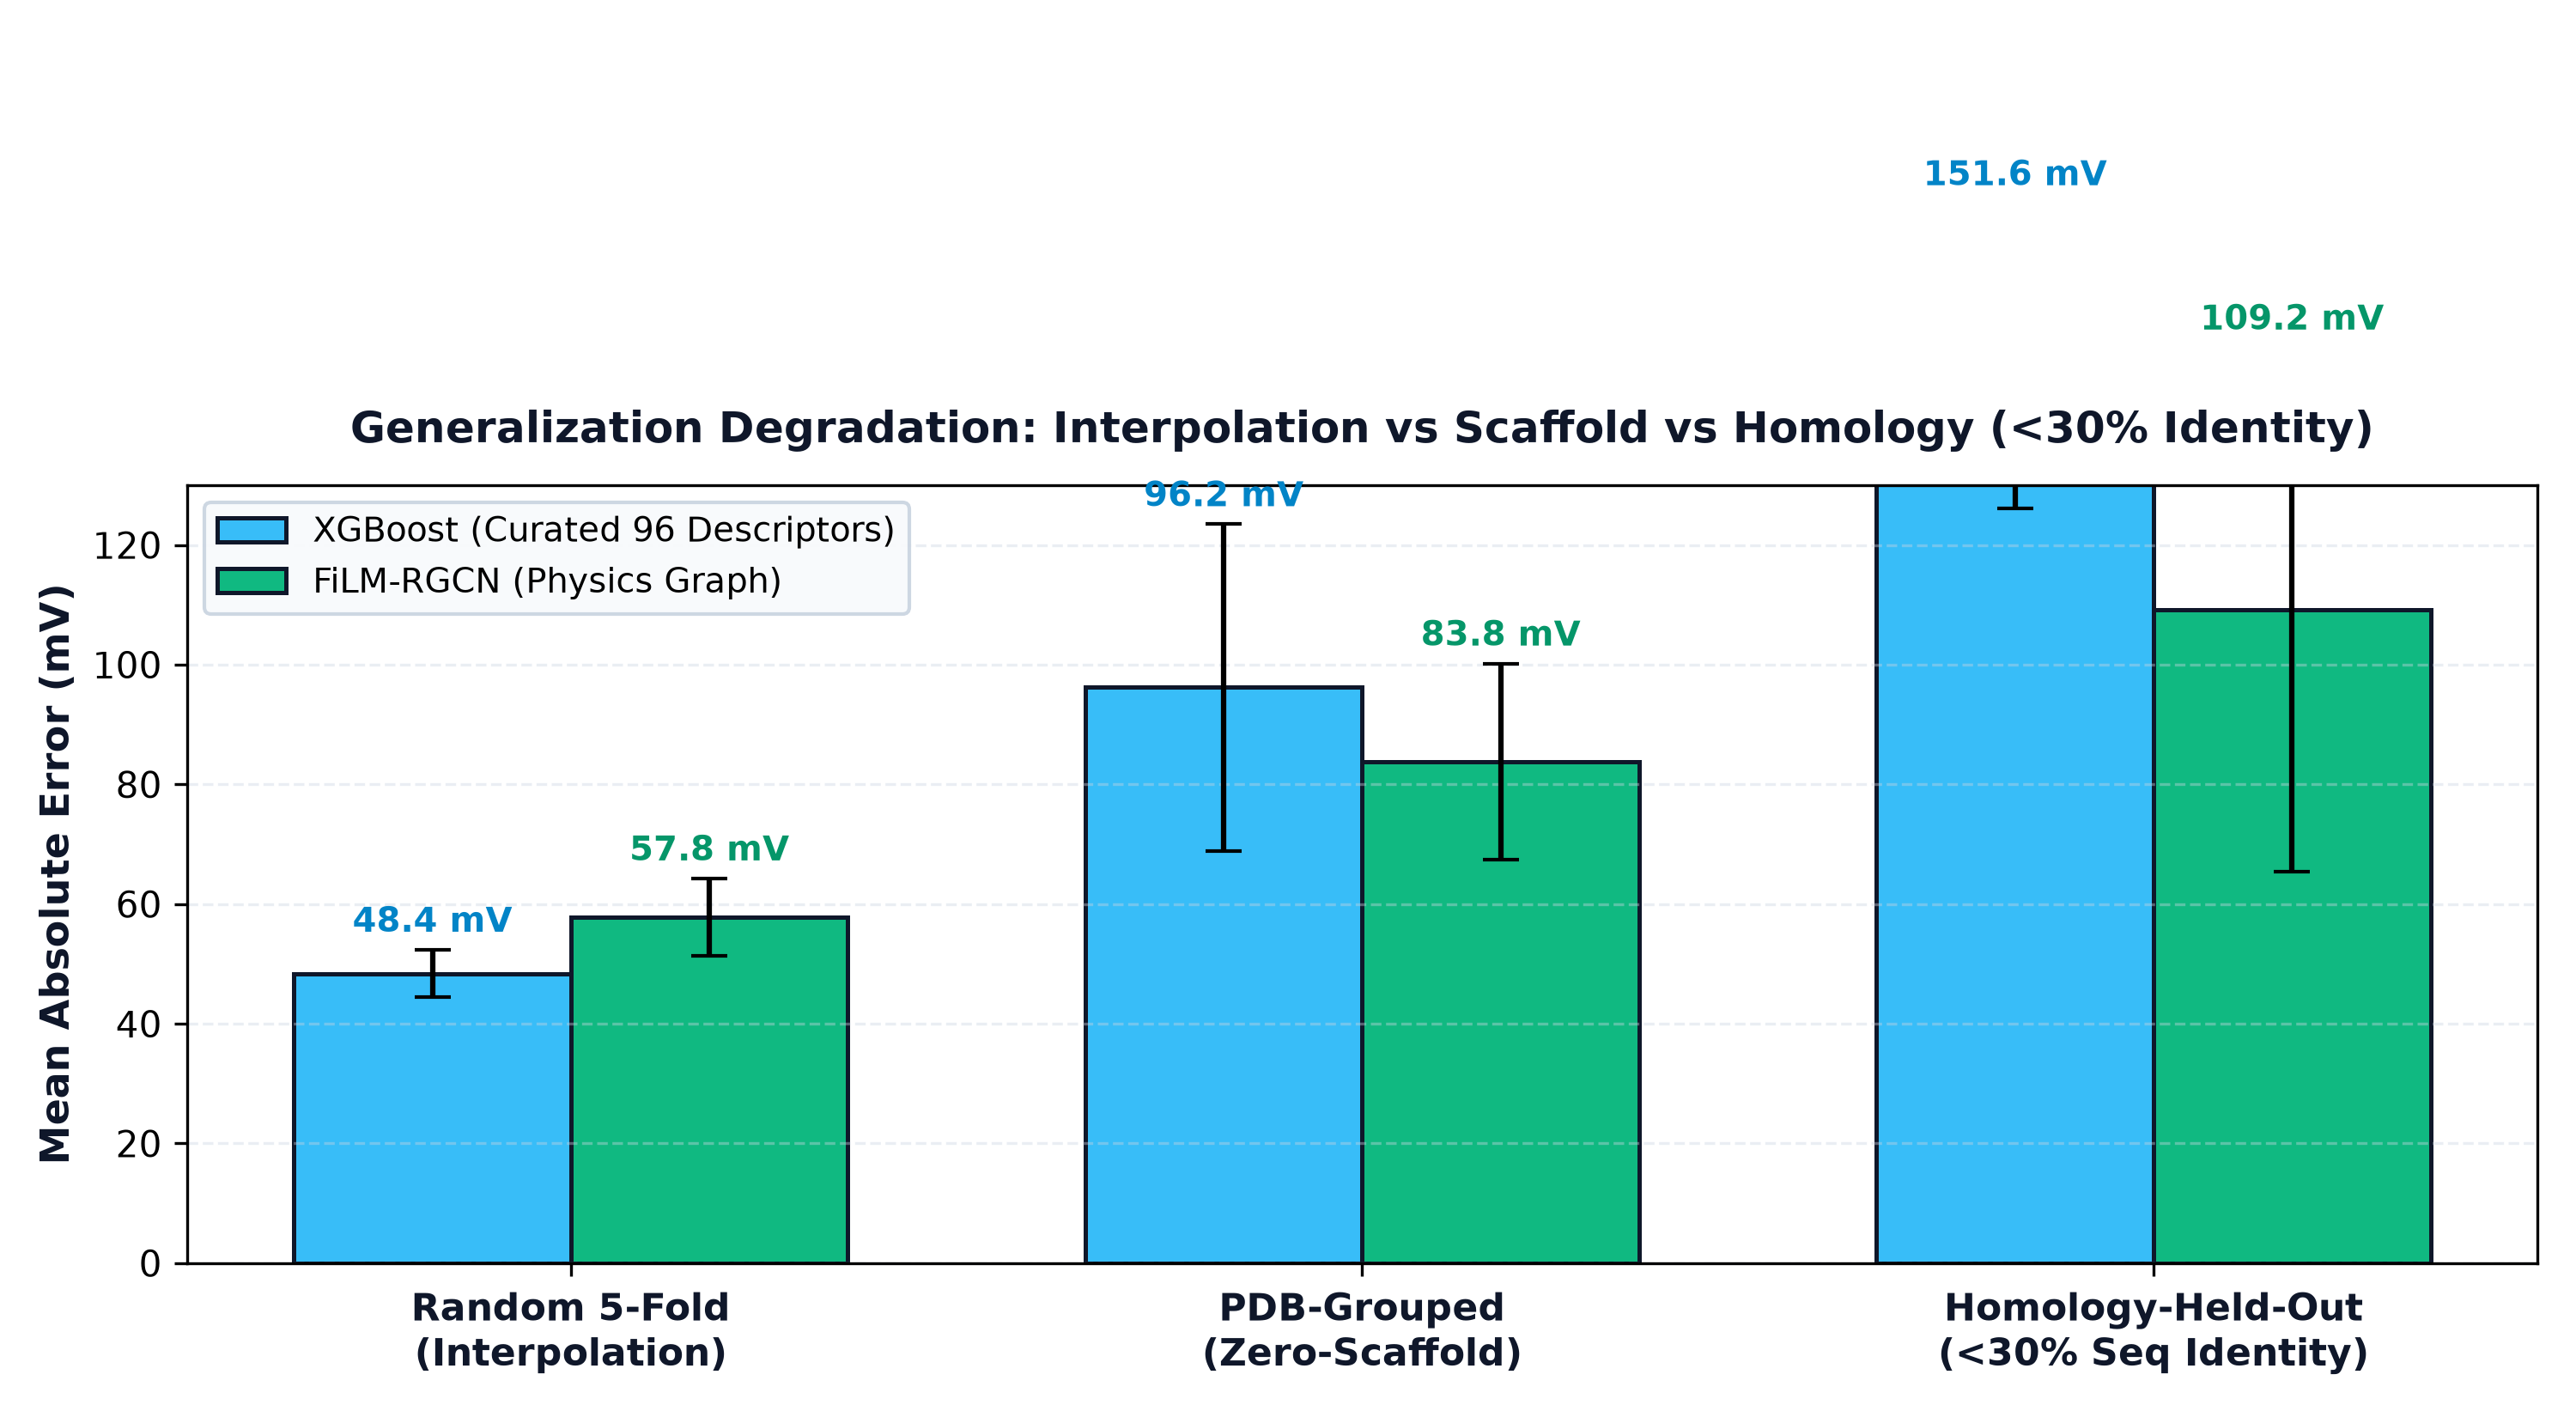
\includegraphics[width=\textwidth]{fig2_generalization_benchmark.png}
\caption{Comparison of Curated XGBoost versus FiLM-RGCN across three validation regimes. (A) Mean Absolute Error (MAE) under Random 5-Fold, PDB-Grouped (zero base-scaffold leakage), and Sequence-Homology-Held-Out ($<30\%$ sequence identity) cross-validation; error bars denote standard deviation across cross-validation splits. (B) Out-of-fold parity scatter plot for FiLM-RGCN on sequence-homology-held-out splits ($r = 0.820$).}
\label{fig:generalization}
\end{figure}

The relative performance of the two architectures depended strongly on the validation regime:
\begin{itemize}
    \item \textbf{Random 5-Fold:} Curated XGBoost performed better than FiLM-RGCN ($48.39\text{ mV}$ vs $57.83\text{ mV}$ MAE), consistent with the efficiency of gradient-boosted trees on tabular descriptors under dense interpolation.
    \item \textbf{PDB-Grouped:} When base crystal scaffolds were held out strictly blind, Curated XGBoost error increased by $+47.8\text{ mV}$ to $96.20 \pm 27.29\text{ mV}$. FiLM-RGCN error increased by $+26.0\text{ mV}$ to $83.82 \pm 16.38\text{ mV}$, outperforming XGBoost by $12.38\text{ mV}$ with an approximately $40\%$ lower fold-to-fold standard deviation ($16.38\text{ mV}$ vs $27.29\text{ mV}$).
    \item \textbf{Sequence-Homology-Held-Out:} Under strict sequence-identity constraints ($<30\%$ pairwise identity), XGBoost degraded to an MAE of $151.59 \pm 25.53\text{ mV}$ ($R^2 = 0.474$, $r = 0.717$). FiLM-RGCN reported an MAE of $109.18 \pm 43.82\text{ mV}$ ($R^2 = 0.654$, $r = 0.820$), achieving a $42.41\text{ mV}$ lower error.
\end{itemize}

While a paired $t$-test across the cross-validation folds showed a nominally significant difference ($p = 0.0031$), standard fold-level tests violate independence assumptions due to overlapping training sets across splits. Therefore, this result should be interpreted as favoring FiLM-RGCN under the evaluated partitions rather than as definitive parametric inference [ADD GROUP-AWARE STATISTICAL COMPARISON]. Tabular models rely on combinations of global scalar descriptors that do not transfer reliably to distinct sequences, whereas multi-relational residue graphs maintain more consistent performance across sequence disconnect.

\subsection{Mechanistic Edge and pH Ablations}
Targeted ablation experiments were performed under the standardized 100-epoch schedule across matched 5-fold splits (Supporting Information Table~S1):
\begin{enumerate}
    \item \textbf{Solvent pH Conditioning:} Removing pH conditioning entirely increased MAE by $+17.29\text{ mV}$ (from $58.45\text{ mV}$ to $75.74 \pm 6.94\text{ mV}$, $R^2 = 0.787$). Randomly shuffling pH values produced a similar degradation ($76.27 \pm 7.87\text{ mV}$, $R^2 = 0.796$). This confirms that the model actively uses pH. However, this ablation demonstrates that pH is an informative feature; it does not prove that layer-wise FiLM modulation is superior to appending pH at the readout layer [READOUT-ONLY-PH CONTROL REQUIRED].
    \item \textbf{Relational Edge Types:} Removing Type 2 putative polar contact edges ($\text{N}\cdots\text{O} \le 3.5\text{ \AA}$) increased MAE by $+3.57\text{ mV}$ to $62.02 \pm 6.36\text{ mV}$ ($R^2 = 0.866$). Removing Type 3 cysteine sulfur proximities ($\text{S}_\gamma\cdots\text{S}_\gamma \le 2.5\text{ \AA}$) increased MAE by $+4.76\text{ mV}$ to $63.21 \pm 8.60\text{ mV}$ ($R^2 = 0.873$).
    \item \textbf{Permutation Controls:} Randomly permuting residue node feature vectors degraded MAE to $66.24 \pm 5.62\text{ mV}$ ($R^2 = 0.855$), and scrambling relation labels degraded MAE to $66.34 \pm 7.08\text{ mV}$ ($R^2 = 0.848$).
\end{enumerate}

\subsection{Graph-Connectivity Sensitivity Analysis}
To examine model sensitivity to structural connectivity without retraining, we performed in-silico edge perturbation sweeps on four representative crystal structures (\texttt{4FXC}, \texttt{1AYF}, \texttt{1FXA}, \texttt{6RXN}) by adjusting distance thresholds for Type 2 polar contacts between $3.0\text{ \AA}$ and $4.2\text{ \AA}$ (Supporting Information Figure~S1) [VERIFY PERTURBATION PROTOCOL DETAILS].

In all four scaffolds, reducing polar contact edges initially increased the predicted reduction potential ($\Delta \widehat{E}_m > 0$, peaking between $+40$ and $+120\text{ mV}$ at $3.8\text{--}3.9\text{ \AA}$), followed by attenuation at higher thresholds where edge-dropout sparsifies message-passing pathways. We note that this response is an in-silico sensitivity analysis of graph connectivity, not a physical simulation of structural relaxation. Furthermore, the non-monotonic response curve reflects non-linear interactions across convolutional layers rather than direct validation of a physical mechanism.

\subsection{Mutational Shift ($\Delta E_m$) Prediction as a Methodological Limitation}
To assess whether the model captures the energetic consequences of sequence mutations, out-of-fold cross-validation predictions were evaluated for all $N = 233$ wild-type/mutant pairs across 28 base crystal scaffolds (Supporting Information Figure~S2) [ADD MUTANT-STRUCTURE GENERATION DETAILS]:
\begin{equation}
\Delta E_m^{\text{pred}} = \widehat{E}_m(\text{mutant}) - \widehat{E}_m(\text{WT})
\end{equation}
Results are summarized in Table~\ref{tab:mutational_validation}.

\begin{table}[htbp]
\centering
\caption{Out-of-Fold Evaluation of Predicted Mutational Shifts ($\Delta E_m$) on $N = 233$ Pairs (28 Base Scaffolds)}
\label{tab:mutational_validation}
\resizebox{\textwidth}{!}{%
\begin{tabular}{lccccc}
\toprule
Model Baseline & MAE (mV) & RMSE (mV) & Pearson $r$ & Spearman $\rho$ & Sign Accuracy \\
\midrule
Null Baseline ($\Delta E_m = 0$) & $\mathbf{54.8}$ & $86.1$ & --- & --- & --- \\
FiLM-RGCN (Sample-Level) & $60.8$ & $\mathbf{82.3}$ & $0.373$ ($p = 4.3 \times 10^{-9}$) & $0.014$ & $42.5\%$ \\
FiLM-RGCN (Scaffold-Bootstrap)\textsuperscript{\emph{a}} & $61.2$ & $82.4$ & $0.282$ ($[-0.198, 0.683]$) & --- & --- \\
\bottomrule
\end{tabular}%
}
\vspace{1ex}
\raggedright
\footnotesize
\textsuperscript{\emph{a}} Clustered bootstrap across 28 unique scaffolds ($10{,}000$ resamples); brackets denote 95\% confidence intervals.
\end{table}

While FiLM-RGCN yields a modest improvement in RMSE relative to the zero-shift baseline ($82.3\text{ mV}$ vs $86.1\text{ mV}$), its MAE is worse ($60.8\text{ mV}$ vs $54.8\text{ mV}$), rank correlation is essentially absent ($\rho = 0.014$), and directional sign accuracy is $42.5\%$ (below random guessing). When accounting for clustered errors across the 28 scaffolds via bootstrap resampling, the 95\% confidence interval for Pearson $r$ spans zero ([$ -0.198, 0.683$], $p = 0.470$).

This limitation arises partly because over $50\%$ of experimental mutations have subtle effects ($|\Delta E_m^{\text{exp}}| \le 30\text{ mV}$), which approaches the typical experimental reproducibility of protein film voltammetry ($\pm 15\text{ to } 30\text{ mV}$).\cite{armstrong1997reactions,armstrong2018protein} However, experimental noise does not fully account for poor directional performance. Consequently, while FiLM-RGCN captures general scale variation, it cannot reliably predict the polarity or rank ordering of point mutations.

\subsection{Cluster Nuclearity Subgroup Analysis}
Performance varies considerably across cluster nuclearity classes (Supporting Information Table~S2):
\begin{itemize}
    \item $[2\text{Fe}--2\text{S}]$ ferredoxins ($N=293$, $80.5\%$): $\text{MAE} = 56.18\text{ mV}$, $\text{RMSE} = 76.89\text{ mV}$, $R^2 = 0.913$, $r = 0.958$.
    \item Rubredoxin $[1\text{Fe}]$ centers ($N=52$, $14.3\%$): $\text{MAE} = 47.91\text{ mV}$, $\text{RMSE} = 63.72\text{ mV}$, $R^2 = 0.540$, $r = 0.752$.
    \item $[4\text{Fe}--4\text{S}]$ clusters ($N=11$, $3.0\%$): $\text{MAE} = 131.51\text{ mV}$, $\text{RMSE} = 169.41\text{ mV}$, $R^2 = 0.352$, $r = 0.629$.
    \item $[3\text{Fe}--4\text{S}]$ clusters ($N=8$, $2.2\%$): $\text{MAE} = 110.77\text{ mV}$, $\text{RMSE} = 156.50\text{ mV}$.
\end{itemize}
These results reflect dataset composition: predictions are reasonably accurate for $[2\text{Fe}--2\text{S}]$ and $[1\text{Fe}]$ proteins, but degrade substantially on $[4\text{Fe}--4\text{S}]$ and $[3\text{Fe}--4\text{S}]$ systems due to data scarcity.

\subsection{Implementation Checks and Uncertainty Calibration}
Across 200 random 3D rotations and translations (50 per scaffold across four structures), maximum prediction discrepancies were $\le 6.10 \times 10^{-5}\text{ mV}$, verifying numerical rigid-body SE(3) invariance (Supporting Information Table~S3). 

Epistemic uncertainty estimated via 50 Monte Carlo Dropout passes yielded nominal 95\% predictive intervals that captured only $\sim 50\%$ of experimental observations (Supporting Information Section~S13). This indicates that uncalibrated dropout is overconfident on out-of-distribution scaffolds, and conformal prediction or calibrated ensembling will be necessary for reliable uncertainty estimates.

\section{Conclusions}
In this study, we developed and evaluated FiLM-RGCN, a pH-conditioned multi-relational residue graph neural network for predicting iron--sulfur protein reduction potentials. Our findings highlight a clear split-dependent trade-off: curated tabular XGBoost models perform better under standard random cross-validation interpolation ($48.39\text{ mV}$ vs $57.83\text{ mV}$ MAE), but FiLM-RGCN demonstrates superior generalization under structural and evolutionary disconnect, outperforming XGBoost on PDB-grouped splits ($83.82\text{ mV}$ vs $96.20\text{ mV}$) and sequence-homology-held-out splits ($109.18\text{ mV}$ vs $151.59\text{ mV}$).

We also documented several key operational boundaries: point-mutation sign accuracy ($42.5\%$) remains below random chance, performance degrades on scarce $[4\text{Fe}--4\text{S}]$ and $[3\text{Fe}--4\text{S}]$ clusters, and single-model dropout uncertainty is under-dispersed. Addressing these challenges through explicit cofactor coordination representations, physics-informed protonation modeling, and calibrated ensemble methods will be important directions for future work.

\section*{Supporting Information}
The Supporting Information is available free of charge at \url{https://pubs.acs.org}.
Complete feature audit details, physicochemical descriptor parameters, graph construction distributions, hyperparameter optimization protocols, sequence alignment identity matrices, full ablation tables, multi-point pH titration fits, in-silico edge perturbation curves, mutational shift bootstrap analyses, cluster nuclearity breakdowns, and uncertainty calibration curves.

\section*{Data and Code Availability}
Curated benchmark datasets, structural coordinates, model weights, and reproduction scripts are available at: \url{https://github.com/hubdk17/Redox_Potential} [INSERT FINAL REPOSITORY DOI/URL].

\begin{acknowledgement}
The authors acknowledge computational infrastructure support. [ANONYMIZED FOR PEER REVIEW].
\end{acknowledgement}

\bibliography{references}

\end{document}
